% Graph Representations and Depth-First Search -- Metropolis beamer slides
% Compile: pdflatex graphs-dfs.tex (x2)
\documentclass[10pt,aspectratio=169]{beamer}

\usetheme{metropolis}
\metroset{block=fill, numbering=fraction, progressbar=frametitle}

\usepackage[T1]{fontenc}
\usepackage{amsmath, amssymb}
\usepackage{listings}
\usepackage{booktabs}
\usepackage{tikz}
\usetikzlibrary{arrows.meta, positioning, calc}

% ---- colors -------------------------------------------------------------
\definecolor{mLightBlue}{HTML}{4C72B0}
\definecolor{mGreen}{HTML}{55A868}
\definecolor{mRed}{HTML}{C44E52}
\definecolor{mGray}{HTML}{BFBFBF}
\setbeamercolor{alerted text}{fg=mRed}

% ---- code style ---------------------------------------------------------
\lstdefinestyle{jl}{
  basicstyle=\ttfamily\footnotesize,
  keywordstyle=\color{mRed}\bfseries,
  commentstyle=\color{mGreen}\itshape,
  numberstyle=\tiny\color{mGray},
  showstringspaces=false,
  breaklines=true,
  columns=fullflexible,
  morekeywords={function,for,in,if,else,elseif,end,return,length,while}
}
\lstset{style=jl}

% ---- graph helpers ------------------------------------------------------
\tikzset{
  vtx/.style={draw, circle, minimum size=7mm, inner sep=0pt, font=\small,
              fill=white},
  seen/.style={vtx, fill=mLightBlue!35},
  done/.style={vtx, fill=mGreen!35},
  edg/.style={thick, mGray!80!black},
  dedg/.style={edg, -{Stealth[length=2.5mm]}},
  tree/.style={very thick, mLightBlue},
  wlbl/.style={fill=white, inner sep=1.5pt, font=\scriptsize},
}

% ---- title --------------------------------------------------------------
\title{Graphs and Depth-First Search}
\subtitle{Representations, DFS, Components, Pre/Post Numbers, Topological Sort, Cycles}
\date{}
\author{}

\begin{document}

\maketitle

% =========================================================================
\begin{frame}{Graphs}
  A \alert{graph} $G = (V, E)$ is a set of vertices $V$ and a set of edges $E$.
  Throughout,
  \[
    n = |V|, \qquad m = |E|.
  \]

  \pause
  \bigskip
  Graphs model \alert{pairwise relationships}:
  \begin{itemize}
    \item the web: pages are vertices, links are edges;
    \item social networks: people are vertices, friendships are edges;
    \item road maps, flight routes, biological networks, \ldots
  \end{itemize}
\end{frame}

\begin{frame}{Four Kinds of Graphs}
  \begin{center}
  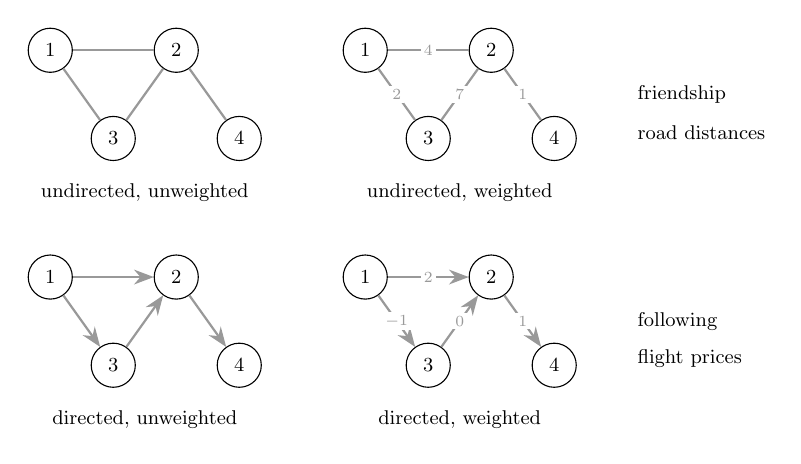
\begin{tikzpicture}[scale=0.8, every node/.style={transform shape}]
    \begin{scope}
      \node[vtx] (1) at (0,0) {1}; \node[vtx] (2) at (2,0) {2};
      \node[vtx] (3) at (1,-1.4) {3}; \node[vtx] (4) at (3,-1.4) {4};
      \draw[edg] (1) -- (2); \draw[edg] (1) -- (3);
      \draw[edg] (2) -- (3); \draw[edg] (2) -- (4);
      \node[below] at (1.5,-2.0) {\small undirected, unweighted};
    \end{scope}
    \begin{scope}[xshift=5cm]
      \node[vtx] (1) at (0,0) {1}; \node[vtx] (2) at (2,0) {2};
      \node[vtx] (3) at (1,-1.4) {3}; \node[vtx] (4) at (3,-1.4) {4};
      \draw[edg] (1) -- node[wlbl] {4} (2); \draw[edg] (1) -- node[wlbl] {2} (3);
      \draw[edg] (2) -- node[wlbl] {7} (3); \draw[edg] (2) -- node[wlbl] {1} (4);
      \node[below] at (1.5,-2.0) {\small undirected, weighted};
    \end{scope}
    \begin{scope}[yshift=-3.6cm]
      \node[vtx] (1) at (0,0) {1}; \node[vtx] (2) at (2,0) {2};
      \node[vtx] (3) at (1,-1.4) {3}; \node[vtx] (4) at (3,-1.4) {4};
      \draw[dedg] (1) -- (2); \draw[dedg] (1) -- (3);
      \draw[dedg] (3) -- (2); \draw[dedg] (2) -- (4);
      \node[below] at (1.5,-2.0) {\small directed, unweighted};
    \end{scope}
    \begin{scope}[xshift=5cm, yshift=-3.6cm]
      \node[vtx] (1) at (0,0) {1}; \node[vtx] (2) at (2,0) {2};
      \node[vtx] (3) at (1,-1.4) {3}; \node[vtx] (4) at (3,-1.4) {4};
      \draw[dedg] (1) -- node[wlbl] {2} (2); \draw[dedg] (1) -- node[wlbl] {$-1$} (3);
      \draw[dedg] (3) -- node[wlbl] {0} (2); \draw[dedg] (2) -- node[wlbl] {1} (4);
      \node[below] at (1.5,-2.0) {\small directed, weighted};
    \end{scope}
    \node[right, align=left] at (9.2,-0.7) {\small friendship};
    \node[right, align=left] at (9.2,-1.3) {\small road distances};
    \node[right, align=left] at (9.2,-4.3) {\small following};
    \node[right, align=left] at (9.2,-4.9) {\small flight prices};
  \end{tikzpicture}
  \end{center}
\end{frame}

% =========================================================================
\section{Graph Representations}

\begin{frame}{Adjacency Matrix}
  An $n \times n$ matrix with $A[i,j]$ = weight of edge $i \to j$, or
  $\emptyset$ if there is none. Undirected graphs have $A[i,j] = A[j,i]$.

  \bigskip
  \begin{columns}[c]
    \begin{column}{0.4\textwidth}
      \begin{center}
      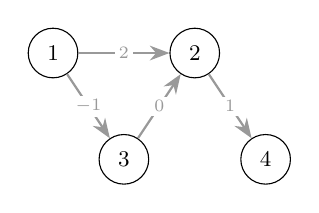
\begin{tikzpicture}[scale=0.9, every node/.style={transform shape}]
        \node[vtx] (1) at (0,0) {1}; \node[vtx] (2) at (2,0) {2};
        \node[vtx] (3) at (1,-1.5) {3}; \node[vtx] (4) at (3,-1.5) {4};
        \draw[dedg] (1) -- node[wlbl] {2} (2); \draw[dedg] (1) -- node[wlbl] {$-1$} (3);
        \draw[dedg] (3) -- node[wlbl] {0} (2); \draw[dedg] (2) -- node[wlbl] {1} (4);
      \end{tikzpicture}
      \end{center}
    \end{column}
    \begin{column}{0.5\textwidth}
      \[
        A = \begin{bmatrix}
          \emptyset & 2 & -1 & \emptyset \\
          \emptyset & \emptyset & \emptyset & 1 \\
          \emptyset & 0 & \emptyset & \emptyset \\
          \emptyset & \emptyset & \emptyset & \emptyset
        \end{bmatrix}
      \]
    \end{column}
  \end{columns}

  \bigskip
  \pause
  \begin{itemize}
    \item Space: $O(n^2)$, wasteful when the graph is \alert{sparse}.
    \item Is there an edge $i \to j$? $O(1)$.
  \end{itemize}
\end{frame}

\begin{frame}[fragile]{Adjacency Matrix in Julia}
  Use \texttt{Inf} for ``no edge'':

  \bigskip
\begin{lstlisting}
A = [
    Inf   2.0  -1.0  Inf;
    Inf   Inf   Inf   1.0;
    Inf   0.0   Inf   Inf;
    Inf   Inf   Inf   Inf
]
\end{lstlisting}

  \bigskip
  \begin{center}
    Row $i$ lists what vertex $i$ points to. Most entries are \texttt{Inf}.
  \end{center}
\end{frame}

\begin{frame}[fragile]{Adjacency List}
  For each vertex, store the list of its neighbours. For weighted graphs, store
  pairs $(v, w)$: neighbour and edge weight.

  \bigskip
  \begin{columns}[c]
    \begin{column}{0.4\textwidth}
      \[
        \begin{aligned}
          L[1] &= \{(2,\ 2),\ (3,\ {-1})\} \\
          L[2] &= \{(4,\ 1)\} \\
          L[3] &= \{(2,\ 0)\} \\
          L[4] &= \emptyset
        \end{aligned}
      \]
    \end{column}
    \begin{column}{0.55\textwidth}
\begin{lstlisting}
L = [
    [(2, 2), (3, -1)],  # vertex 1
    [(4, 1)],           # vertex 2
    [(2, 0)],           # vertex 3
    []                  # vertex 4
]
\end{lstlisting}
    \end{column}
  \end{columns}

  \bigskip
  \pause
  \begin{itemize}
    \item Space: $O(n + m)$, proportional to the size of the graph.
    \item Is there an edge $u \to v$? $O(\deg(u))$: scan $L[u]$.
  \end{itemize}
\end{frame}

\begin{frame}{Matrix or List?}
  \begin{center}
  \begin{tabular}{lcc}
    \toprule
                         & matrix   & list \\
    \midrule
    space                & $O(n^2)$ & $O(n + m)$ \\
    is $u \to v$ an edge? & $O(1)$   & $O(\deg(u))$ \\
    list neighbours of $u$ & $O(n)$  & $O(\deg(u))$ \\
    \bottomrule
  \end{tabular}
  \end{center}

  \bigskip
  \begin{center}
    Real graphs are usually sparse ($m \ll n^2$), and traversals only ever
    ask for neighbours.\\[4pt]
    \alert{We use adjacency lists from now on.}
  \end{center}
\end{frame}

% =========================================================================
\section{Depth-First Search}

\begin{frame}[fragile]{Depth-First Search}
  Starting from a source vertex, go as \alert{deep} as possible along each
  branch, and \alert{backtrack} only when stuck.

  \bigskip
\begin{lstlisting}
visited = falses(n)

function visit(adj, s)
    visited[s] = true             # mark s as visited
    for v in adj[s]               # for weighted graphs: for (v, _) in adj[s]
        if !visited[v]
            visit(adj, v)         # go deeper
        end
    end
end                               # every neighbour handled: backtrack
\end{lstlisting}
\end{frame}

% ---- DFS trace ----------------------------------------------------------
\begin{frame}{DFS in Action}
  Call \texttt{visit(adj, 1)}, scanning neighbours in increasing order.

  \bigskip
  \begin{columns}[c]
    \begin{column}{0.5\textwidth}
      \begin{center}
      \begin{tikzpicture}[scale=1.0, every node/.style={transform shape}]
        \coordinate (p1) at (0,0);    \coordinate (p2) at (1.8,0.9);
        \coordinate (p3) at (1.8,-0.9); \coordinate (p4) at (3.6,0);
        \coordinate (p5) at (5.2,0.9);  \coordinate (p6) at (5.2,-0.9);
        \draw[edg] (p1) -- (p2); \draw[edg] (p1) -- (p3);
        \draw[edg] (p2) -- (p4); \draw[edg] (p3) -- (p4);
        \draw[edg] (p4) -- (p5); \draw[edg] (p5) -- (p6);
        \only<3->{\draw[tree] (p1) -- (p2);}
        \only<4->{\draw[tree] (p2) -- (p4);}
        \only<5->{\draw[tree] (p4) -- (p3);}
        \only<6->{\draw[tree] (p4) -- (p5);}
        \only<7->{\draw[tree] (p5) -- (p6);}
        \foreach \i in {1,...,6} \node[vtx] at (p\i) {\i};
        \only<2->{\node[seen] at (p1) {1};}
        \only<3->{\node[seen] at (p2) {2};}
        \only<4->{\node[seen] at (p4) {4};}
        \only<5->{\node[seen] at (p3) {3};}
        \only<6->{\node[seen] at (p5) {5};}
        \only<7->{\node[seen] at (p6) {6};}
      \end{tikzpicture}
      \end{center}
    \end{column}
    \begin{column}{0.45\textwidth}
      \small
      \begin{itemize}
        \item<2-> visit 1
        \item<3-> 1's first neighbour 2: visit 2
        \item<4-> 2's neighbours 1, 4: visit 4
        \item<5-> 4's neighbours 2, 3, 5: visit 3\\
              3 has nothing new: \alert{backtrack} to 4
        \item<6-> visit 5
        \item<7-> visit 6, then backtrack all the way
      \end{itemize}
    \end{column}
  \end{columns}

  \bigskip
  \onslide<8->{
  \begin{center}
    Visit order $1, 2, 4, 3, 5, 6$. The \textcolor{mLightBlue}{blue} edges
    form the \alert{DFS tree}; edge $1$--$3$ is never followed.
  \end{center}}
\end{frame}

\begin{frame}{Running Time}
  \begin{itemize}
    \item Each vertex is marked once, so \texttt{visit} is called at most
          $n$ times: $O(n)$.
    \pause
    \bigskip
    \item The call \texttt{visit(adj, s)} scans the list \texttt{adj[s]}
          once. Over all vertices,
          \[
            \sum_{s \in V} \deg(s) =
            \begin{cases}
              m  & \text{directed}, \\
              2m & \text{undirected},
            \end{cases}
          \]
          so the scanning costs $O(m)$.
  \end{itemize}

  \pause
  \bigskip
  \begin{alertblock}{}
    \centering DFS runs in $O(n + m)$ time: linear in the size of the graph.
  \end{alertblock}
\end{frame}

\begin{frame}{Reachability}
  \textbf{Question.} Which vertices can be reached from $s$?

  \bigskip
  \textbf{Answer.} Call \texttt{visit(adj, s)}. Afterwards,
  \[
    \texttt{visited[v]} = \texttt{true}
    \quad\Longleftrightarrow\quad
    \text{there is a path from } s \text{ to } v.
  \]

  \bigskip
  \pause
  \begin{itemize}
    \item ($\Rightarrow$) DFS only moves along edges, so it only marks
          vertices it can walk to from $s$.
    \item ($\Leftarrow$) If some reachable $v$ stayed unmarked, take the first
          unmarked vertex on a path $s \leadsto v$. Its predecessor on the path
          was marked, and its scan would have visited it. Contradiction.
  \end{itemize}
\end{frame}

% =========================================================================
\section{Connected Components}

\begin{frame}{Connected Components}
  A \alert{connected component} of an undirected graph is a maximal set of
  vertices in which every pair is joined by a path.

  \bigskip
  \begin{center}
  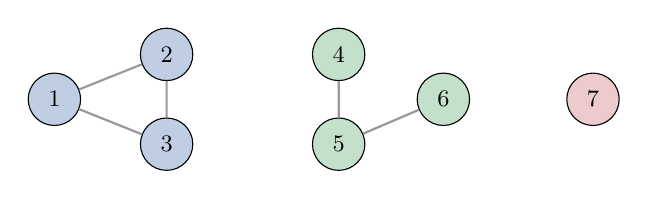
\begin{tikzpicture}[scale=0.95, every node/.style={transform shape}]
    \node[seen] (1) at (0,0) {1}; \node[seen] (2) at (1.5,0.6) {2};
    \node[seen] (3) at (1.5,-0.6) {3};
    \draw[edg] (1) -- (2); \draw[edg] (1) -- (3); \draw[edg] (2) -- (3);
    \node[done] (4) at (3.8,0.6) {4}; \node[done] (5) at (3.8,-0.6) {5};
    \node[done] (6) at (5.2,0) {6};
    \draw[edg] (4) -- (5); \draw[edg] (5) -- (6);
    \node[vtx, fill=mRed!30] (7) at (7.2,0) {7};
  \end{tikzpicture}
  \end{center}

  \bigskip
  \begin{center}
    Three components: $\{1,2,3\}$, $\{4,5,6\}$, $\{7\}$.
  \end{center}

  \pause
  \bigskip
  \textbf{Key observation.} \texttt{visit(adj, s)} marks exactly the vertices
  reachable from $s$, which is exactly \alert{the component of $s$}.
\end{frame}

\begin{frame}{Counting Components}
  Scan the vertices. Each time we find one not yet visited, it starts a new
  component: launch a fresh DFS from it.

  \bigskip
  \begin{center}
  \begin{tabular}{l}
    $\textit{counter} \gets 0$ \\
    \textbf{for} each vertex $v \in V$: \\
    \quad \textbf{if not} \texttt{visited[v]}: \\
    \quad\quad $\textit{counter} \gets \textit{counter} + 1$ \\
    \quad\quad \texttt{visit(adj, v)}
  \end{tabular}
  \end{center}

  \bigskip
  \pause
  \begin{itemize}
    \item Each \texttt{visit} from the outer loop marks one whole component.
    \item Across \emph{all} the calls, every vertex is visited once and every
          list is scanned once: still $O(n + m)$.
  \end{itemize}
\end{frame}

\begin{frame}[fragile]{Connected Components in Julia}
\begin{lstlisting}[basicstyle=\ttfamily\scriptsize]
function connected_components(n, adj)
    visited = falses(n)
    component = zeros(Int, n)      # component[v] = label of v's component
    num_components = 0
    function visit(s)
        visited[s] = true
        component[s] = num_components
        for v in adj[s]
            if !visited[v]
                visit(v)
            end
        end
    end
    for s in 1:n
        if !visited[s]
            num_components += 1
            visit(s)
        end
    end
    return num_components, component
end
\end{lstlisting}
\end{frame}

% =========================================================================
\section{Pre and Post Numbers}

\begin{frame}{Pre and Post Numbers}
  Augment DFS with a global \alert{clock} that ticks up by 1 each time it is read.

  \bigskip
  For each vertex $v$ record:
  \begin{itemize}
    \item $\mathrm{pre}[v]$: clock value when $v$ is \alert{first visited}.
    \item $\mathrm{post}[v]$: clock value when $v$ \alert{finishes} (all descendants processed).
  \end{itemize}

  \bigskip
  \begin{center}
    The interval $[\mathrm{pre}[v],\, \mathrm{post}[v]]$ spans the entire time $v$
    is on the call stack.
  \end{center}
\end{frame}

\begin{frame}[fragile]{Computing Pre and Post Numbers}
\begin{lstlisting}
clock   = 1
pre     = zeros(Int, n)
post    = zeros(Int, n)
visited = falses(n)

function visit(adj, s)
    visited[s] = true
    pre[s] = clock;  clock += 1          # s first seen
    for v in adj[s]
        if !visited[v]
            visit(adj, v)
        end
    end
    post[s] = clock;  clock += 1         # s finishes
end
\end{lstlisting}
\end{frame}

\begin{frame}{Pre/Post Example}
  Run DFS on this DAG from vertex 1, visiting neighbours in order.

  \bigskip
  \begin{columns}[c]
    \begin{column}{0.38\textwidth}
      \begin{center}
      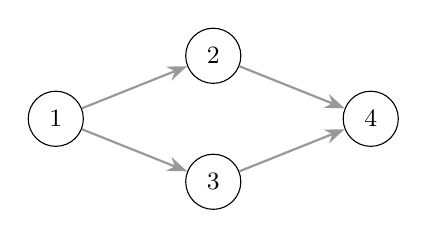
\begin{tikzpicture}[scale=1.0, every node/.style={transform shape}]
        \node[vtx] (1) at (0, 0)   {1};
        \node[vtx] (2) at (2, 0.8) {2};
        \node[vtx] (3) at (2,-0.8) {3};
        \node[vtx] (4) at (4, 0)   {4};
        \draw[dedg] (1) -- (2);
        \draw[dedg] (1) -- (3);
        \draw[dedg] (2) -- (4);
        \draw[dedg] (3) -- (4);
      \end{tikzpicture}
      \end{center}
    \end{column}
    \begin{column}{0.55\textwidth}
      \begin{center}
      \begin{tabular}{ccc}
        \toprule
        vertex & $\mathrm{pre}$ & $\mathrm{post}$ \\
        \midrule
        1 & 1 & 8 \\
        2 & 2 & 5 \\
        3 & 6 & 7 \\
        4 & 3 & 4 \\
        \bottomrule
      \end{tabular}
      \end{center}

      \bigskip
      Order of events: pre(1), pre(2), pre(4), post(4), post(2), pre(3), post(3), post(1).
    \end{column}
  \end{columns}
\end{frame}

\begin{frame}{Post Numbers and Topological Order}
  \begin{block}{Key Property}
    In a DAG, for every edge $u \to v$: \quad $\mathrm{post}[u] > \mathrm{post}[v]$.
  \end{block}

  \bigskip
  \textbf{Why.} When DFS traverses $u \to v$ there are two cases:
  \begin{itemize}
    \item $v$ is \alert{not yet visited}: DFS recurses into $v$, finishes $v$
          completely, then returns to $u$. So $\mathrm{post}[v] < \mathrm{post}[u]$.
    \item $v$ is \alert{already finished}: $\mathrm{post}[v]$ was assigned before
          DFS even started $u$, so $\mathrm{post}[v] < \mathrm{pre}[u] < \mathrm{post}[u]$.
  \end{itemize}
  (A back edge $u \to v$ where $v$ is on the stack $\Rightarrow$ cycle $\Rightarrow$
  impossible in a DAG.)
\end{frame}

\begin{frame}{Post Numbers and Topological Order: Visualization}
  Each vertex's active interval $[\mathrm{pre},\mathrm{post}]$ on the clock:

  \bigskip
  \begin{center}
  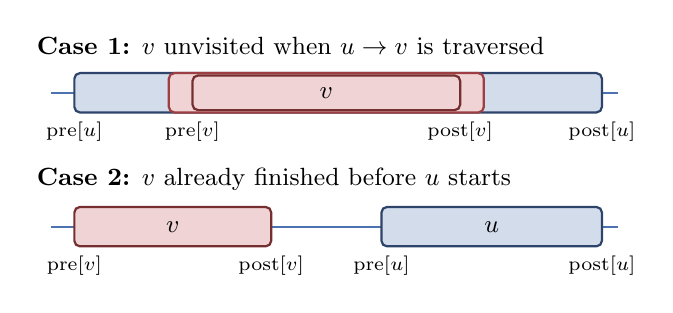
\begin{tikzpicture}[scale=1.0]
    % Case 1: v nested inside u
    \node[anchor=west, font=\small] at (-0.3, 1.6) {\textbf{Case 1:} $v$ unvisited when $u \to v$ is traversed};
    \draw[thick, mLightBlue] (0, 1.0) -- (7.2, 1.0);
    \draw[thick, mLightBlue!60!black, fill=mLightBlue!25, rounded corners=2pt]
      (0.3, 0.75) rectangle (7.0, 1.25);
    \node[font=\small] at (3.65, 1.0) {$u$};
    \draw[thick, mRed!80!black, fill=mRed!25, rounded corners=2pt]
      (1.5, 0.75) rectangle (5.5, 1.25);
    \node[font=\small] at (3.5, 1.0) {};
    \draw[thick, mRed!60!black, fill=mRed!25, rounded corners=2pt]
      (1.8, 0.78) rectangle (5.2, 1.22);
    \node[font=\small] at (3.5, 1.0) {$v$};
    \node[font=\scriptsize, below] at (0.3,  0.75) {$\mathrm{pre}[u]$};
    \node[font=\scriptsize, below] at (1.8,  0.75) {$\mathrm{pre}[v]$};
    \node[font=\scriptsize, below] at (5.2,  0.75) {$\mathrm{post}[v]$};
    \node[font=\scriptsize, below] at (7.0,  0.75) {$\mathrm{post}[u]$};

    % Case 2: v entirely before u
    \node[anchor=west, font=\small] at (-0.3, -0.1) {\textbf{Case 2:} $v$ already finished before $u$ starts};
    \draw[thick, mLightBlue] (0, -0.7) -- (7.2, -0.7);
    \draw[thick, mRed!60!black, fill=mRed!25, rounded corners=2pt]
      (0.3, -0.95) rectangle (2.8, -0.45);
    \node[font=\small] at (1.55, -0.7) {$v$};
    \draw[thick, mLightBlue!60!black, fill=mLightBlue!25, rounded corners=2pt]
      (4.2, -0.95) rectangle (7.0, -0.45);
    \node[font=\small] at (5.6, -0.7) {$u$};
    \node[font=\scriptsize, below] at (0.3, -0.95) {$\mathrm{pre}[v]$};
    \node[font=\scriptsize, below] at (2.8, -0.95) {$\mathrm{post}[v]$};
    \node[font=\scriptsize, below] at (4.2, -0.95) {$\mathrm{pre}[u]$};
    \node[font=\scriptsize, below] at (7.0, -0.95) {$\mathrm{post}[u]$};
  \end{tikzpicture}
  \end{center}

  \bigskip
  \begin{center}
    In both cases $\mathrm{post}[v] < \mathrm{post}[u]$, so sorting by \alert{decreasing} post gives a topological order.
  \end{center}
\end{frame}

% =========================================================================
\section{Topological Sorting}

\begin{frame}{Topological Sorting}
  A \alert{topological order} of a directed graph lists the vertices so that
  every edge $u \to v$ has $u$ \alert{before} $v$.

  \bigskip
  Think of tasks with dependencies: $u \to v$ means $u$ must be done before
  $v$.

  \bigskip
  \begin{center}
  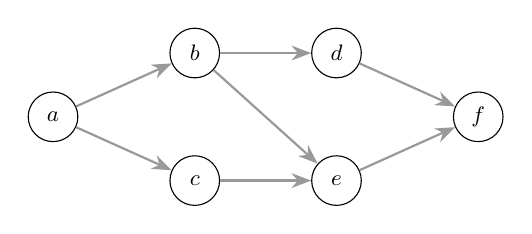
\begin{tikzpicture}[scale=0.9, every node/.style={transform shape}]
    \node[vtx] (a) at (0,0) {$a$};    \node[vtx] (b) at (2,0.9) {$b$};
    \node[vtx] (c) at (2,-0.9) {$c$}; \node[vtx] (d) at (4,0.9) {$d$};
    \node[vtx] (e) at (4,-0.9) {$e$}; \node[vtx] (f) at (6,0) {$f$};
    \draw[dedg] (a) -- (b); \draw[dedg] (a) -- (c); \draw[dedg] (b) -- (d);
    \draw[dedg] (c) -- (e); \draw[dedg] (d) -- (f); \draw[dedg] (e) -- (f);
    \draw[dedg] (b) -- (e);
  \end{tikzpicture}
  \end{center}
\end{frame}

\begin{frame}{One Valid Order}
  Lay the vertices out as $a, b, c, d, e, f$:

  \bigskip
  \begin{center}
  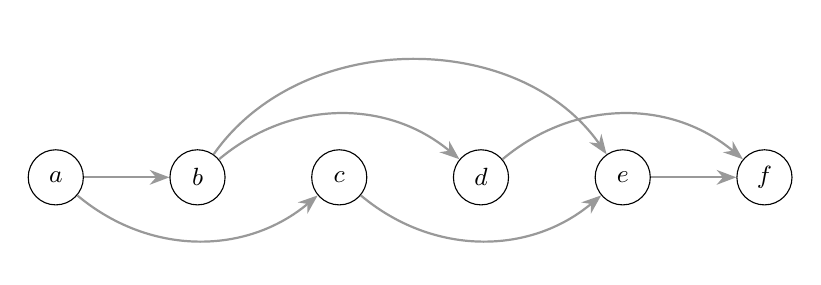
\begin{tikzpicture}[scale=1.0, every node/.style={transform shape}]
    \foreach \x/\l in {0/a, 1.8/b, 3.6/c, 5.4/d, 7.2/e, 9.0/f}
      \node[vtx] (\l) at (\x,0) {$\l$};
    \draw[dedg] (a) -- (b);
    \draw[dedg] (e) -- (f);
    \draw[dedg] (b) to[bend left=40] (d);
    \draw[dedg] (b) to[bend left=55] (e);
    \draw[dedg] (d) to[bend left=40] (f);
    \draw[dedg] (a) to[bend right=40] (c);
    \draw[dedg] (c) to[bend right=40] (e);
  \end{tikzpicture}
  \end{center}

  \bigskip
  \begin{center}
    Every edge points \alert{left to right}.
  \end{center}
\end{frame}

\begin{frame}{Only DAGs Have One}
  \begin{block}{Fact}
    A directed graph with a cycle has \alert{no} topological order.
  \end{block}

  \bigskip
  If $v_1 \to v_2 \to \cdots \to v_k \to v_1$ is a cycle, a topological order
  would need
  \[
    v_1 \text{ before } v_2 \text{ before } \cdots \text{ before } v_k
    \text{ before } v_1.
  \]
  Contradiction.

  \bigskip
  \pause
  So we only sort \alert{directed acyclic graphs} (DAGs). Every DAG has a
  topological order, and DFS finds one.
\end{frame}

\begin{frame}[fragile]{The Algorithm}
  Since higher post numbers come first, prepend each vertex when it
  \alert{finishes} — equivalent to sorting by decreasing post number, but in $O(n + m)$.

\begin{lstlisting}[basicstyle=\ttfamily\scriptsize]
visited    = falses(n)
topo_order = Int[]

function visit(adj, s)
    visited[s] = true
    for v in adj[s]
        if !visited[v]
            visit(adj, v)
        end
    end
    pushfirst!(topo_order, s)    # s finishes: prepend it
end

for s in 1:n
    if !visited[s]
        visit(adj, s)
    end
end
\end{lstlisting}
\end{frame}

\begin{frame}{Trace}
  DFS from $a$, neighbours in alphabetical order.

  \begin{columns}[c]
    \begin{column}{0.45\textwidth}
      \begin{center}
      \begin{tikzpicture}[scale=0.85, every node/.style={transform shape}]
        \node[vtx] (a) at (0,0) {$a$};    \node[vtx] (b) at (2,0.9) {$b$};
        \node[vtx] (c) at (2,-0.9) {$c$}; \node[vtx] (d) at (4,0.9) {$d$};
        \node[vtx] (e) at (4,-0.9) {$e$}; \node[vtx] (f) at (6,0) {$f$};
        \draw[dedg] (a) -- (b); \draw[dedg] (a) -- (c); \draw[dedg] (b) -- (d);
        \draw[dedg] (c) -- (e); \draw[dedg] (d) -- (f); \draw[dedg] (e) -- (f);
        \draw[dedg] (b) -- (e);
        \only<2->{\node[done] at (f) {$f$};}
        \only<3->{\node[done] at (d) {$d$};}
        \only<4->{\node[done] at (e) {$e$};}
        \only<5->{\node[done] at (b) {$b$};}
        \only<6->{\node[done] at (c) {$c$};}
        \only<7->{\node[done] at (a) {$a$};}
      \end{tikzpicture}
      \end{center}
    \end{column}
    \begin{column}{0.5\textwidth}
      \small
      \begin{tabular}{ll}
        \toprule
        event & \texttt{topo\_order} \\
        \midrule
        \uncover<2->{$a \to b \to d \to f$, $f$ finishes & $[f]$} \\
        \uncover<3->{$d$ finishes & $[d, f]$} \\
        \uncover<4->{$b \to e$ ($f$ done), $e$ finishes & $[e, d, f]$} \\
        \uncover<5->{$b$ finishes & $[b, e, d, f]$} \\
        \uncover<6->{$a \to c$ ($e$ done), $c$ finishes & $[c, b, e, d, f]$} \\
        \uncover<7->{$a$ finishes & $[a, c, b, e, d, f]$} \\
        \bottomrule
      \end{tabular}
    \end{column}
  \end{columns}

  \onslide<7->{
  \begin{center}
    Check: every edge goes left to right in $a, c, b, e, d, f$.
  \end{center}}
\end{frame}

\begin{frame}{Why It Works}
  \begin{block}{Claim}
    In a DAG, every edge $u \to v$ has $v$ finishing \alert{before} $u$, so
    $u$ is placed in front of $v$.
  \end{block}

  \bigskip
  Look at the moment DFS scans the edge $u \to v$ inside \texttt{visit(u)}.
  \begin{itemize}
    \item \textbf{$v$ not yet visited.} We call \texttt{visit(v)} and it
          returns before $u$ finishes.
    \pause
    \item \textbf{$v$ already finished.} Then $v$ finished first. Done.
    \pause
    \item \textbf{$v$ visited but not finished.} Then $v$ is still on the
          call stack below $u$, so there is a path $v \leadsto u$. With
          $u \to v$ that is a \alert{cycle}: impossible in a DAG.
  \end{itemize}

  \pause
  \bigskip
  \begin{center}
    One DFS over the whole graph: $O(n + m)$.
  \end{center}
\end{frame}

% ---------------------------------------------------------------- exercise
\begin{frame}{Exercise}
  \begin{center}
    Run the DFS algorithm (neighbours in increasing order, outer loop
    $1, \ldots, 5$) and give the topological order it produces.
  \end{center}

  \bigskip
  \begin{center}
  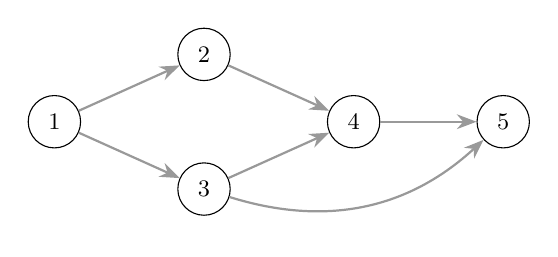
\begin{tikzpicture}[scale=0.95, every node/.style={transform shape}]
    \node[vtx] (1) at (0,0) {1};    \node[vtx] (2) at (2,0.9) {2};
    \node[vtx] (3) at (2,-0.9) {3}; \node[vtx] (4) at (4,0) {4};
    \node[vtx] (5) at (6,0) {5};
    \draw[dedg] (1) -- (2); \draw[dedg] (1) -- (3); \draw[dedg] (2) -- (4);
    \draw[dedg] (3) -- (4); \draw[dedg] (4) -- (5);
    \draw[dedg] (3) to[bend right=30] (5);
  \end{tikzpicture}
  \end{center}
\end{frame}

\begin{frame}{Solution}
  \begin{itemize}
    \item $1 \to 2 \to 4 \to 5$: finish $5$, then $4$, then $2$.
    \item Back at $1$: $1 \to 3$. Both $4$ and $5$ are done, so $3$
          finishes, then $1$.
  \end{itemize}

  \bigskip
  Finish order $5, 4, 2, 3, 1$. Reversed:
  \begin{center}
  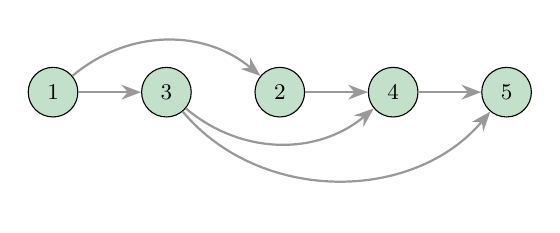
\begin{tikzpicture}[scale=0.9, every node/.style={transform shape}]
    \foreach \x/\l in {0/1, 1.6/3, 3.2/2, 4.8/4, 6.4/5}
      \node[done] (n\l) at (\x,0) {\l};
    \draw[dedg] (n1) to[bend left=40] (n2);
    \draw[dedg] (n1) -- (n3);
    \draw[dedg] (n3) to[bend right=40] (n4);
    \draw[dedg] (n3) to[bend right=50] (n5);
    \draw[dedg] (n2) -- (n4);
    \draw[dedg] (n4) -- (n5);
  \end{tikzpicture}
  \end{center}

  \bigskip
  \begin{center}
    \small $1, 2, 3, 4, 5$ is also valid. A DAG can have many topological
    orders.
  \end{center}
\end{frame}

% =========================================================================
\section{Detecting Cycles}

\begin{frame}[fragile]{Pre and Post Numbers}
  Keep a clock. Stamp each vertex when DFS \alert{enters} it ($pre$) and when
  it \alert{leaves} it ($post$).

  \bigskip
\begin{lstlisting}
time = 1

function visit(adj, s)
    pre[s] = time;  time += 1
    visited[s] = true
    for v in adj[s]
        if !visited[v]
            visit(adj, v)
        end
    end
    post[s] = time; time += 1
end
\end{lstlisting}

  \bigskip
  \begin{center}
    $[pre[v], post[v]]$ is the time interval $v$ spends on the call stack.
  \end{center}
\end{frame}

\begin{frame}{Intervals Nest}
  \begin{columns}[c]
    \begin{column}{0.4\textwidth}
      \begin{center}
      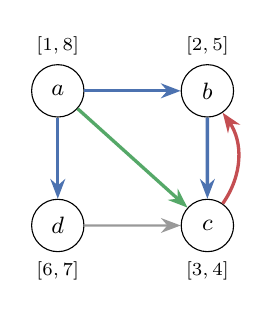
\begin{tikzpicture}[scale=0.95, every node/.style={transform shape}]
        \node[vtx] (a) at (0,0) {$a$};      \node[vtx] (b) at (2,0) {$b$};
        \node[vtx] (c) at (2,-1.8) {$c$};   \node[vtx] (d) at (0,-1.8) {$d$};
        \draw[dedg, tree] (a) -- (b);
        \draw[dedg, tree] (b) -- (c);
        \draw[dedg, tree] (a) -- (d);
        \draw[dedg, mGreen, very thick] (a) -- (c);
        \draw[dedg, mRed, very thick] (c) to[bend right=35] (b);
        \draw[dedg] (d) -- (c);
        \node[font=\scriptsize, above] at (a.north) {$[1,8]$};
        \node[font=\scriptsize, above] at (b.north) {$[2,5]$};
        \node[font=\scriptsize, below] at (c.south) {$[3,4]$};
        \node[font=\scriptsize, below] at (d.south) {$[6,7]$};
      \end{tikzpicture}
      \end{center}
    \end{column}
    \begin{column}{0.55\textwidth}
      \begin{center}
      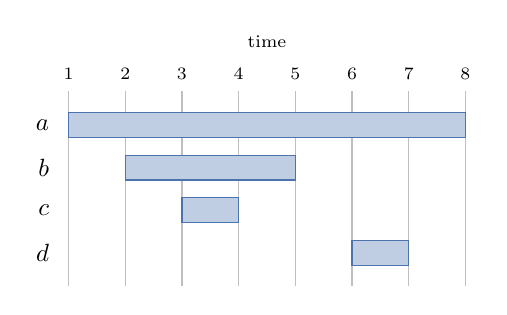
\begin{tikzpicture}[scale=0.9, every node/.style={transform shape}]
        \foreach \t in {1,...,8} {
          \draw[mGray] (\t*0.8-0.8,0.25) -- (\t*0.8-0.8,-2.5);
          \node[font=\scriptsize] at (\t*0.8-0.8,0.5) {\t};
        }
        \foreach \v/\a/\b/\y in {a/1/8/0, b/2/5/1, c/3/4/2, d/6/7/3} {
          \fill[mLightBlue!35, draw=mLightBlue] (\a*0.8-0.8,-\y*0.6-0.05) rectangle (\b*0.8-0.8,-\y*0.6-0.4);
          \node[left] at (-0.15,-\y*0.6-0.225) {$\v$};
        }
        \node[font=\scriptsize] at (2.8,0.95) {time};
      \end{tikzpicture}
      \end{center}
    \end{column}
  \end{columns}

  \bigskip
  DFS from $a$, neighbours in alphabetical order. Two intervals are either
  \alert{nested} (one vertex is a descendant of the other) or
  \alert{disjoint}. They never partially overlap.
\end{frame}

\begin{frame}{Classifying Edges}
  For an edge $u \to v$:

  \bigskip
  \begin{center}
  \begin{tabular}{lll}
    \toprule
    edge type & intervals & example \\
    \midrule
    \textcolor{mLightBlue}{tree} / \textcolor{mGreen}{forward}
      & $pre[u] < pre[v] < post[v] < post[u]$ & $a \to b$, \ $a \to c$ \\
    \textcolor{mRed}{back}
      & $pre[v] < pre[u] < post[u] < post[v]$ & $c \to b$ \\
    cross
      & $pre[v] < post[v] < pre[u] < post[u]$ & $d \to c$ \\
    \bottomrule
  \end{tabular}
  \end{center}

  \bigskip
  \begin{itemize}
    \item Tree edge: DFS discovers $v$ through it. Forward edge: $v$ is a
          descendant found another way.
    \item Back edge: $v$ is an \alert{ancestor} of $u$, still on the stack.
  \end{itemize}

  \pause
  \medskip
  \begin{alertblock}{}
    \centering Only back edges have $post[u] < post[v]$.
  \end{alertblock}
\end{frame}

\begin{frame}{Cycles and Back Edges}
  \begin{block}{Claim}
    A directed graph has a cycle $\iff$ DFS finds a back edge.
  \end{block}

  \medskip
  ($\Leftarrow$) A back edge $u \to v$ means $v$ is an ancestor of $u$ in the
  DFS tree, so there is a path $v \leadsto u$. Adding $u \to v$ closes a
  cycle.

  \pause
  \medskip
  ($\Rightarrow$) Let $v_1 \to v_2 \to \cdots \to v_k \to v_1$ be a cycle, and
  let $v_1$ be the first of its vertices that DFS visits. At that moment the
  rest of the cycle is unvisited, so DFS reaches $v_k$ \alert{before $v_1$
  finishes}:
  \[
    post[v_k] < post[v_1].
  \]
  So the edge $v_k \to v_1$ is a back edge. $\square$
\end{frame}

\begin{frame}[fragile]{Cycle Detection}
  Compute pre/post numbers, then check every edge:
\begin{lstlisting}[basicstyle=\ttfamily\scriptsize]
function has_cycle(n, adj)
    pre, post = dfs_prepost(n, adj)    # DFS from every unvisited vertex
    for u in 1:n
        for v in adj[u]
            if post[u] < post[v]       # back edge
                return true
            end
        end
    end
    return false
end
\end{lstlisting}

  \medskip
  \begin{itemize}
    \item One DFS: $O(n + m)$. One pass over the edges: $O(m)$.
    \item Total: $O(n + m)$.
  \end{itemize}

  \medskip
  \begin{center}
    \small A graph is a DAG exactly when this returns \texttt{false}, so we
    can check before topologically sorting.
  \end{center}
\end{frame}

\end{document}
